
Processes (w no communication) accessing a single DB

Probability of any success =  $p* (1 - p) ^ n-1 $ ...
$p = \Theta(1/n)$ ...
$t = t;$ prob of fail $\leq 1/e$ ...
$t = en*cln(n);$ prob of fail $\leq n^{-c}$ ...
How long until succeeding at least once: $n^{-1}$

The Union bound: Prob [ $\bigcup\limits_{i=1}^{\infty} F_{i}$ ] <= $\sum_{n=1}^{\infty}  Prob[ F_{i}] $ 

%%%%%%%

Verifying AB=C matrix mult

B$\overbar{r} -> A(B\overbar{r})$ and $C\overbar{r}$. if $A(B\overbar{r}) != C\overbar{r}$ then $AB != C$

Principle of Deferred Decisions: If $AB != C$ and $\overbar{r}$ is chosen uniformly at random with $r_n$ at 0-1 then Prob($AB\overbar{r} = C\overbar{r}) <= 1/2$

Law of Total Probability: Let $E_1 ... E_n$ be mutually disjoint events in the sample space $\Omega$ and let $\bigcup\limits_{i=1}^{n} E_{i}$ then $\sum_{i=1}^{n}  Prob[ B | E_{i}] Prob[E_{i}] $ 

Repeated trials increase the runtime to $\Theta(kn^2)$
If it returns false, then it this is right, but if it returns true, then it returns so with some probability of mistake.

%%%%%%%

Average value: $\sum_{j=1}^{\infty}  j * Prob[ X = j ]  = (n + 1) / 2$ while Prob $[X = j] = 1/n$

To take exactly $j$ steps: Prob $[X = j] = (1 - p)^{j - 1} p$
$1/p$ for the first success

Linearity of Expectation: Given 2 random vars $X$ and $Y$ in the same probability space, $E [X + Y] = E[ X ] + E [ Y ] $

Memoryless guessing expected correct: 1, independent of $n$

Memory guessing; $H(n) = \Theta(log(n))$ [harmonic series]

Coupon collection: $E[ X_{j}] = n / (n - j); n $= number of; $j$ = collected; $( n - j ) / n$ of getting a new one
$E[X] = nH(n) = \Theta(nlog(n))$

Conditional Probability: $E[ X | \alpha ] =  \sum_{j=0}^{\infty} j *$ Prob $[ X = j | \alpha]$

For the MAX 3-SAT there is a randomized algo with polynomial expected run time that is guaranteed to produce a truth assignment satisfying at least a $7/8$ fraction of all clauses. We would need $8k$ trials to get the satisfying assignment.

\begin{algorithmic}[1]
	\Function{Select}{$S, k$}
		\State {$a_i \gets random var in S$}
		\For{each element $a_j$ of $S$}
			\State{$S^{-}$.append($a_j$) if $a_j < a_i$}
			\State{$S^{+}$.append($a_j$) if $a_j > a_i$}
		\EndFor
		\If{$S^{-} = k - 1$}
			\State{return $a_i$}
		\ElsIf{$S^{-} \geq k$}
			\State{Select($S^{-}, k$)}
		\Else
			\State{Select($S^{+}, k-1- |S^{-}|$)}
		\EndIf
	\EndFunction
\end{algorithmic}

%%%%
Expected num comparisons  quicksort: $2nln(n) + O(n), \Omega(nlogn)$

%%%

Uniform: Prob $[h(x) = i] = 1/m$ for all $x$ and all $i$
Universal: Prob $[h(x) = h(y)] = 1/m$ for all $x != y$
Near-universal: Prob $[h(x) = h(y)] \leq 2/m$ for all $x != y$; E[$chainLen$] $\leq 2*\alpha;$ Runtime: $\Theta(1 + \alpha)$
k-uniform: Prob $ [ \wedge{}_{j=1}^{k} h(x_j) = i_j) ] = 1 / m^{k}$ for all distinct $x_1...x_k$ and all $i_1...i_k$
Load factor: $\alpha = n/m$
Using balanced binary tree searching is: O(1 + log($chainLen$)) with any hash or O(1 + log($\alpha$)) for uniform
Recursively hash for $O(log_{m}{n})$
Expected search of O(1) with binary probe

%%%%

Formula Satisfiability/SAT: 
$(a \vee b \vee c \vee \overbar{d})$ <=>  $((b \wedge \overbar{c}) \vee \overbar{ ( \overbar{a} => d) } \vee (c \neq a \wedge b)) $

CNF: conjunction/AND of several clauses which use OR inside these clauses.
3CNF: cnf with exactly 3 literals per cllause

Maximum Independent Set (from 3Sat): input is a simple, unweighted graph, get the size of the largest/smallest subgraph
Make the formula into a graph or vice versa, if it has an independent set of size $k$, its possible
Any graph has an edge-complement with the same vertices but the opposite set of edges if its not an edge in $G$. Its independent in $G$ if and only if the same vertices define a clique in $\overbar{G}$ (a complete graph). The largest independent is thus the largest clique in the compliment of the graph.

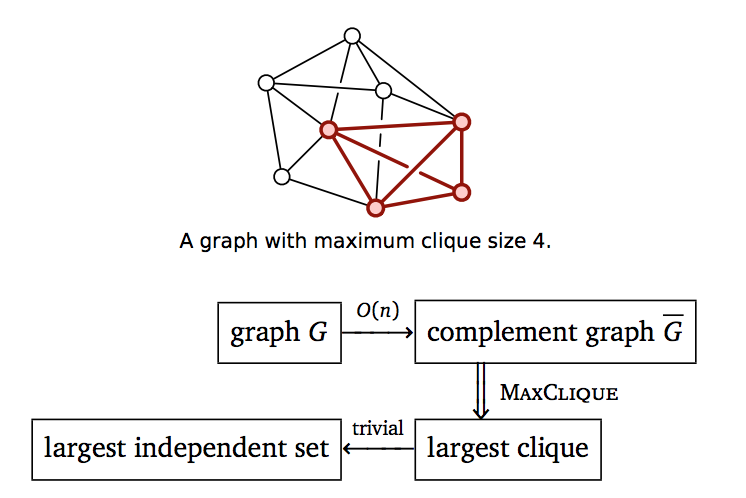
\includegraphics[width=\linewidth]{images/maxclique.png}

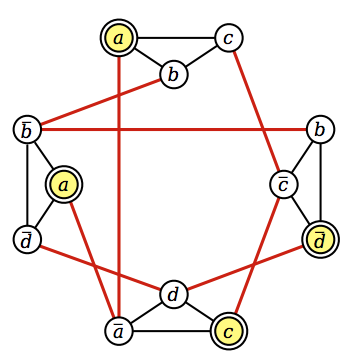
\includegraphics[width=\linewidth]{images/hamcycle.png}

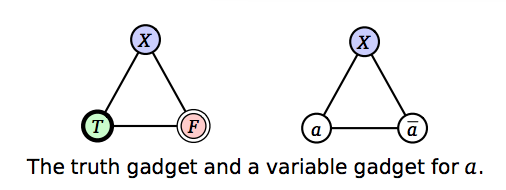
\includegraphics[width=\linewidth]{images/truthgadget.png}

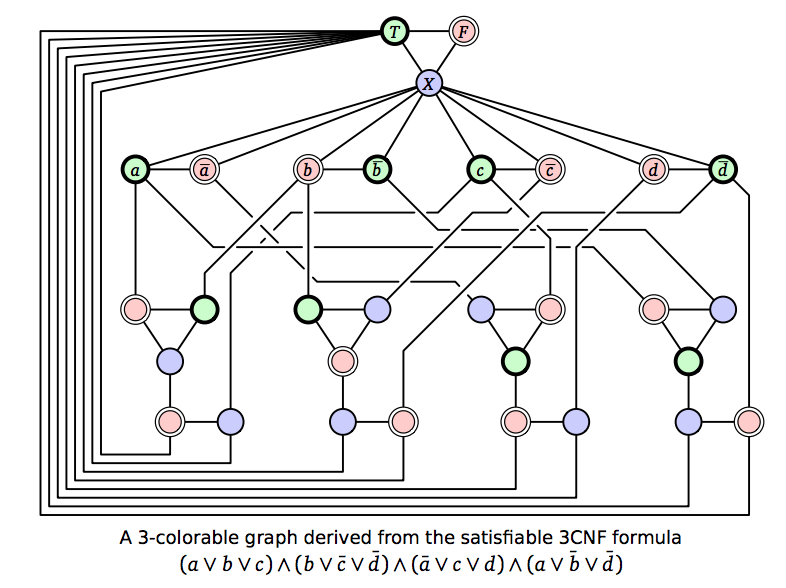
\includegraphics[width=\linewidth]{images/3color.png}


3Color: Truth gadget: $T,F$, and $X$ for true/false/other, variable gadget for variable a connecting and $\overbar{a}$ which must be opposite bools. Clause gadget joining three literal nodes to node $T$ in the truth gadget using give new unlabeled nodes and ten edges.

Hamiltonian Cycle [From Vertex Cover]: For each vertex $u$, all the edge gadgets are connected in $H$ into a single directed path, a vertex chain. $H$ has $d-1$ additional edges for each $i$. $H$ also contains $k$ cover vertices, $1 - k$, with a directed edge to the first vertex in each vertex chain and a directed edge from the last vertex in each vertex chain.
Start at cover vertex 1 and traverse vertex chain for $vu_{2}$, then visit cover vertex 2 and so on and so forth before returning to 1. If $v$ is a part of the vertex cover, follow the edge from $(u_{i}, v, in)$ to $(u_{i}, v, out)$, else, detour from  $(u_{i}, v, in)$ > $(v, u_{i}, in)$ > $(v, u_{i}, out)$ > $(u_{i}, v, out)$.
$G$ contains a vertex cover of size $K$ if and only if $H$ contains a Hamiltonian cycle

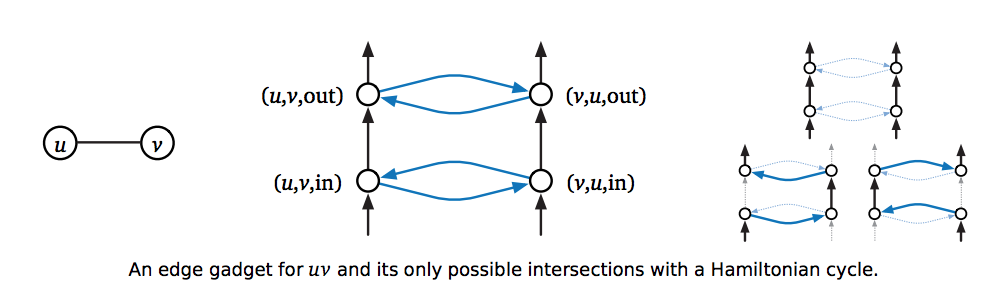
\includegraphics[width=\linewidth]{images/edgegadget.png}


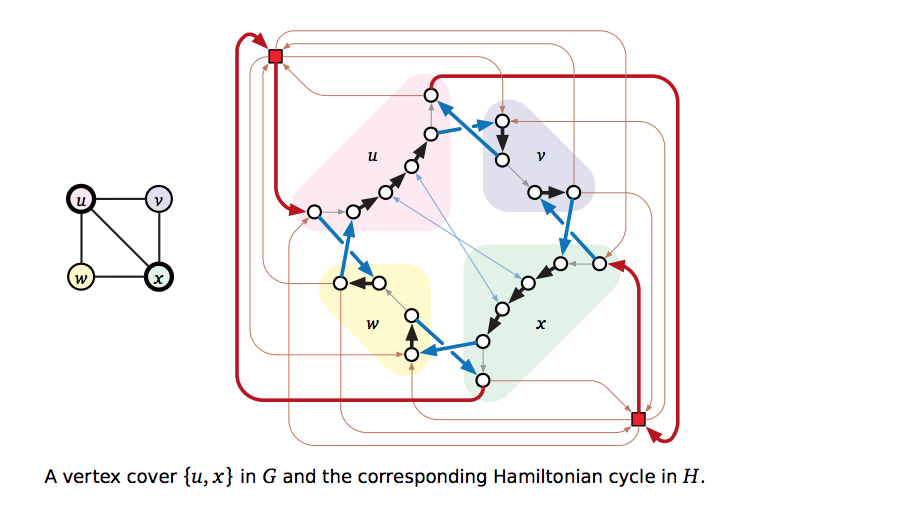
\includegraphics[width=\linewidth]{images/hamiltoniancycle.png}

Subset sum; number edges from 0 to $m-1$; set $X$ contains the integer $b_{i} := f^{i}$ for each edge $i$, and the integer $a_{v} := f^{m} + \sum_{i \delta v}{4^i}$ where $\delta(v)$ is the set of edges that have $v$ as an endpoint. [ $X$ is a $(m+1)$ digit number written in base 4). The $mth$ digit is 1 if vertex, 0 otherwise. $t:= k * 4^m + \sum_{i = 0}^{m-1}{2 * 4^i}$

Draughts: White can capture a certain number of black pieces in a single move if and only if G has a Hamiltonian cycle. Replace edges $uv$ with  $u$-> $v$ and $v$->$u$. If there is a path you can capture them all, if there isn't, you can capture at most 1/2 of them.
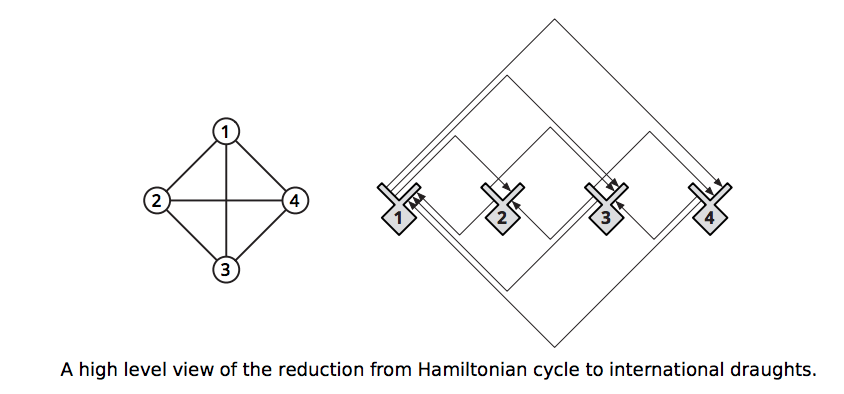
\includegraphics[width=\linewidth]{images/draughtssmall.png}

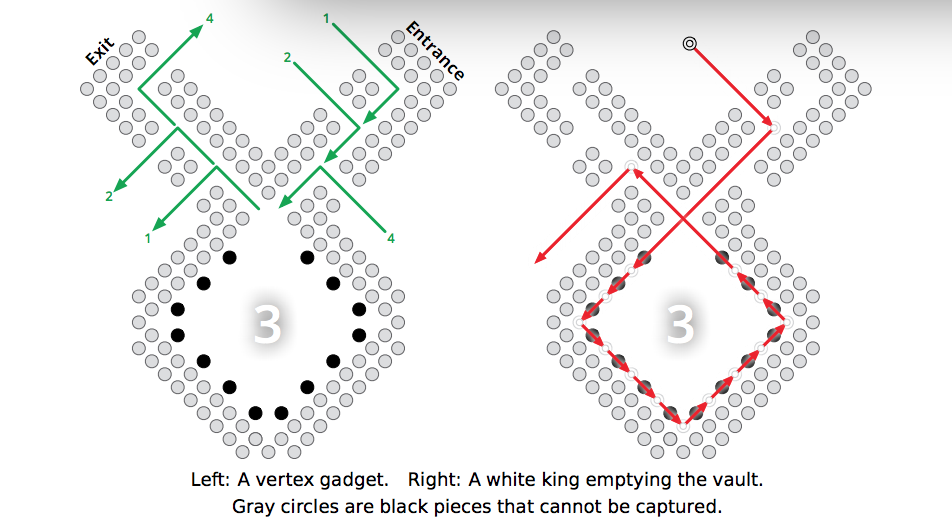
\includegraphics[width=\linewidth]{images/draughts.png}
